\documentclass[12pt]{article}
	\usepackage{amsmath}
	\usepackage{amssymb}
	\usepackage{fancyhdr}
	\usepackage{float}
	\usepackage{graphicx}

	\oddsidemargin0cm
	\topmargin-2cm     %I recommend adding these three lines to increase the 
	\textwidth16.5cm   %amount of usable space on the page (and save trees)
	\textheight23.5cm  

\newcommand{\myname}{Evan Palmer, Titouan Rigoudy}
\newcommand{\myandrew}{esp@andrew, trigoudy@andrew}
\newcommand{\myhwnum}{1}
\newcommand{\problemnum}{1}
\newcommand{\thedate}{\today}
\DeclareMathOperator*{\argmax}{arg\,max}
%Page header
	\setlength{\parindent}{0pt}
	\setlength{\parskip}{5pt plus 1pt}
	 
	\pagestyle{fancyplain}
	\lhead{\fancyplain{}{\textbf{HW\myhwnum}}}      % Note the different brackets!
	\rhead{\fancyplain{}{\myname\\ \myandrew}}
	\chead{\fancyplain{}{15-451 }}
\begin{document}
%Title
	\medskip    
	\thispagestyle{plain}
	\begin{center}                 
	{\LARGE Finding The Best Critic For You} \\
	\medskip
	Machine Learning Midterm Report \\
	\smallskip
	\myname \\
	\myandrew \\
	\thedate \\
	\end{center}
	\vspace{0.5cm}

\section{Introduction}


\section{Obtaining the data}

\section{Data descriptions}

\subsection{Rotten tomatoes}

	The data we retrieved from Rotten tomatoes included approximately five hundred thousand reviews by about four thousand unique critics about four thousand movies.


	\begin{table}[H]
	 \centering
	 \caption{Distribution of number of reviews per critic for movies on rotten tomatoes}
	 \begin{tabular}{ l | c | c | c | c }
	 \hline
	 &  Min & Max & Mean & Std Dev  \\
	 \hline
	 Top Critcs & 0 & 56 & 22.41 & 16.06 \\
	 Other Critics & 0 & 316 & 92.24 & 68.12 \\
	 \hline
	 \end{tabular}
	 \end{table}

	\begin{figure}[H]
	    \centering
	    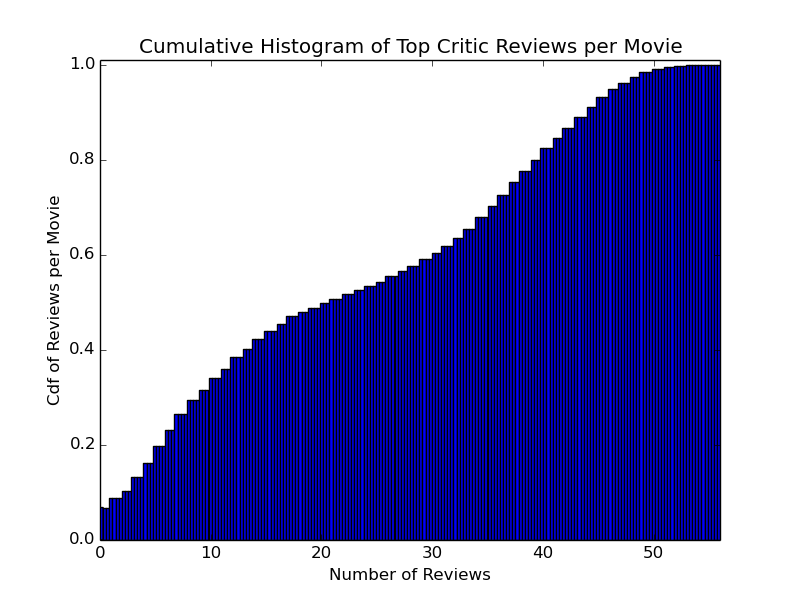
\includegraphics[width=0.48\textwidth]{plots/plot_r_mov_top.png}
	    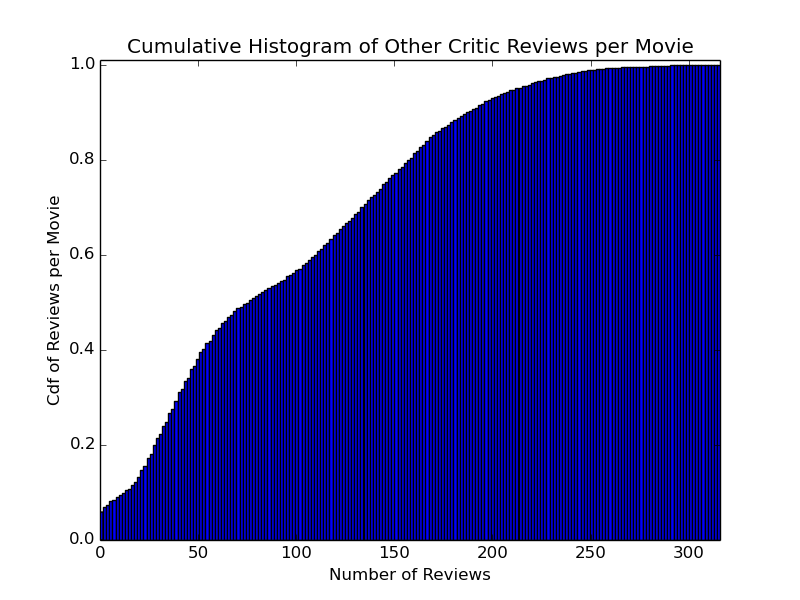
\includegraphics[width=0.48\textwidth]{plots/plot_r_mov_oth.png}
	    \caption{INSERT TITLE}
	    \label{fig:r_mov}
	\end{figure}


	\begin{table}[H]
	 \centering
	 \caption{Distribution of number of reviewed movies per critic on rotten tomatoes} 
	 \begin{tabular}{ l | c | c | c | c }
	 \hline
	 &  Min & Max & Mean & Std Dev  \\
	 \hline
	 Top Critcs & 0 & 2862 & 21.79 & 124.96 \\
	 Other Critics & 0 & 2634 & 68.16 & 224.77 \\
	 \hline
	 \end{tabular}
	 \end{table}

	\begin{figure}[H]
	    \centering
	    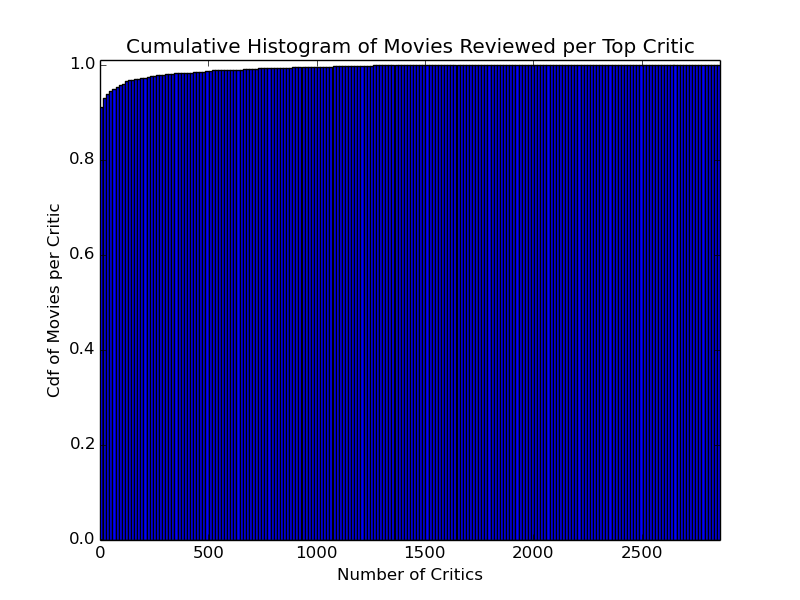
\includegraphics[width=0.48\textwidth]{plots/plot_r_crit_top.png}
	    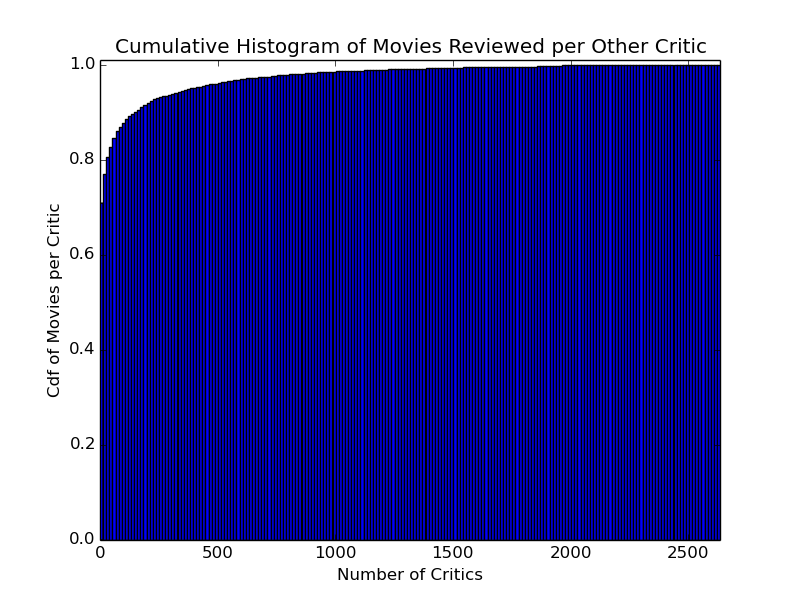
\includegraphics[width=0.48\textwidth]{plots/plot_r_crit_oth.png}
	    \caption{INSERT TITLE}
	    \label{fig:r_crit}
	\end{figure}


	\begin{table}[H]
	 \centering
	 \caption{Distribution of number of reviewed movies per publication on rotten tomatoes} 
	 \begin{tabular}{ l | c | c | c | c }
	 \hline
	 &  Min & Max & Mean & Std Dev  \\
	 \hline
	 Top Publications & 0 & 4135 & 97.22 & 454.15 \\
	 Other Publications & 0 & 3224 & 297.78 & 520.28 \\
	 \hline
	 \end{tabular}
	 \end{table}

	 \begin{figure}[H]
	    \centering
	    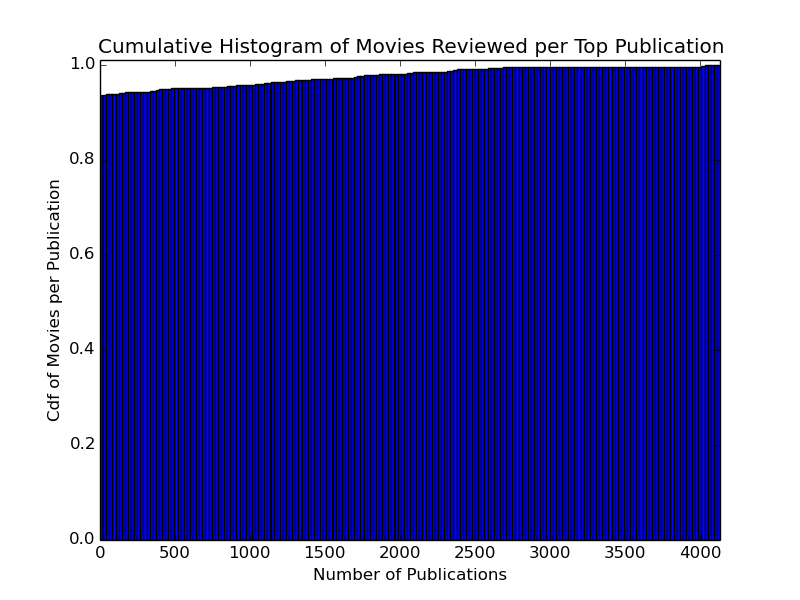
\includegraphics[width=0.48\textwidth]{plots/plot_r_pub_top.png}
	    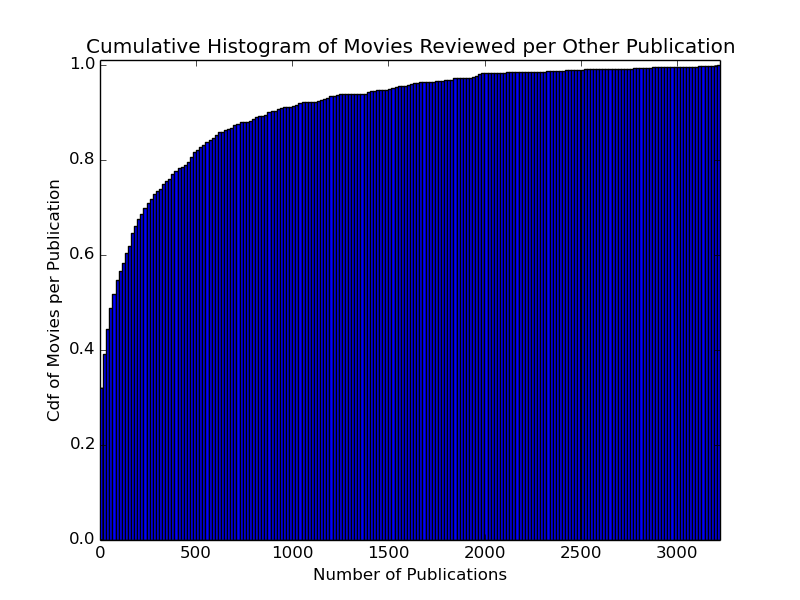
\includegraphics[width=0.48\textwidth]{plots/plot_r_pub_oth.png}
	    \caption{INSERT TITLE}
	    \label{fig:r_pub}
	\end{figure}

\subsection{Metacritic}


	\begin{table}[H]
	 \centering
	 \caption{Distribution of number of reviews by users and critics for movies on metacritic}

	 \begin{tabular}{ l | c | c | c | c }
	 \hline 
	 &  Min & Max & Mean & Std Dev  \\
	 \hline
	 Critics with reviews & 0 & 49 & 25.72 & 10.83 \\
	 Users with reviews & 0 & 842 & 21.56 & 50.05 \\
	 \hline
	 \end{tabular}
	 \end{table}

	 \begin{figure}[H]
	    \centering
	    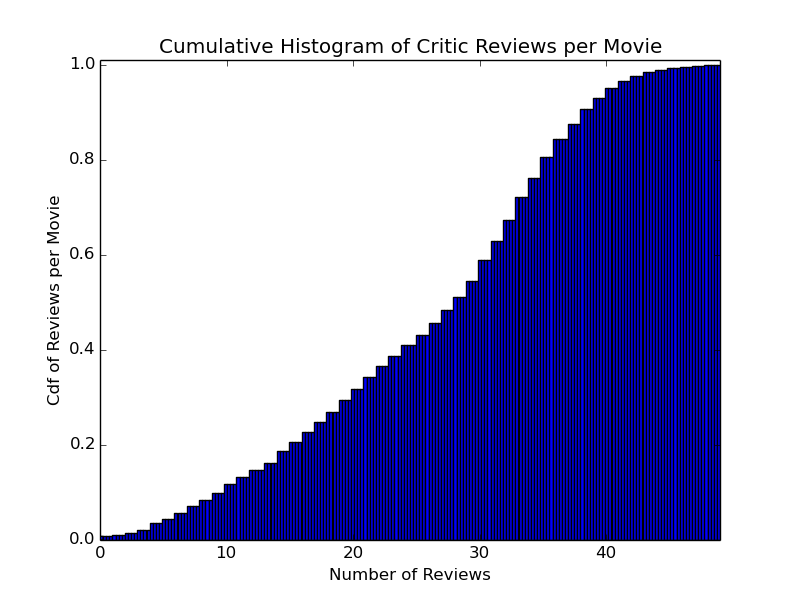
\includegraphics[width=0.48\textwidth]{plots/plot_m_mov_top.png}
	    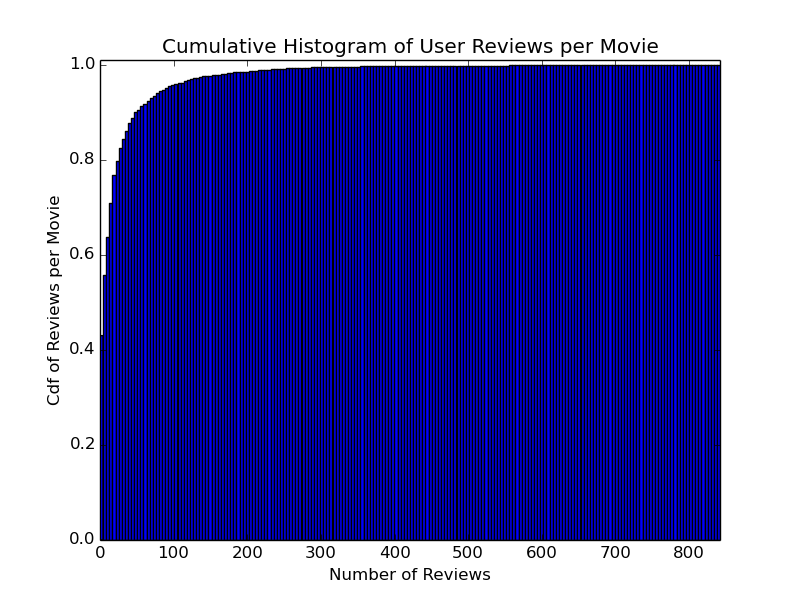
\includegraphics[width=0.48\textwidth]{plots/plot_m_mov_usr.png}
	    \caption{INSERT TITLE}
	    \label{fig:m_mov}
	\end{figure}


	\begin{table}[H]
	\centering
	 \caption{Distribution of number of reviewed movies by users and critics on metacritic}

	 \begin{tabular}{ l | c | c | c | c }
	 \hline
	 &  Min & Max & Mean & Std Dev  \\
	 \hline
	 Reviews per critic & 56 & 3445 & 1203.36 & 912.50 \\
	 Reviews per user & 1 & 536 & 3.45 & 14.55 \\
	 \hline
	 \end{tabular}
	 \end{table}


	 \begin{figure}[H]
	    \centering
	    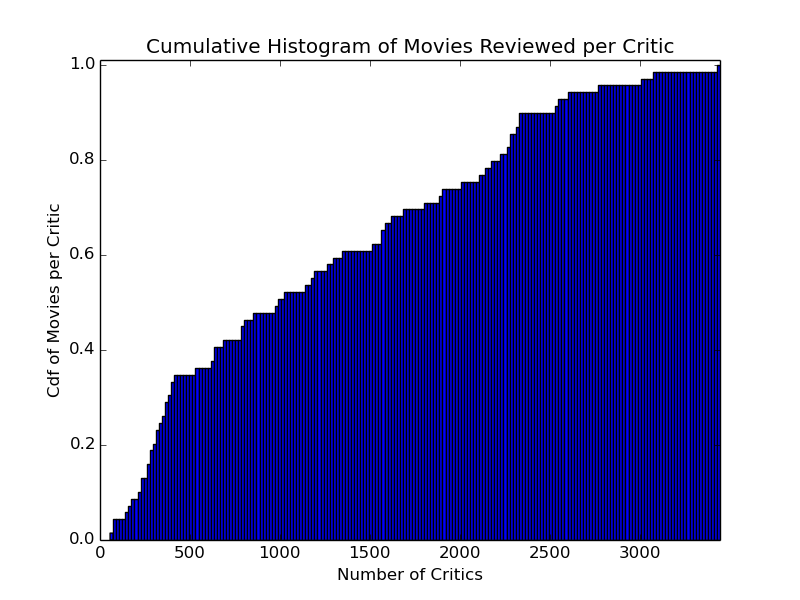
\includegraphics[width=0.48\textwidth]{plots/plot_m_crit_top.png}
	    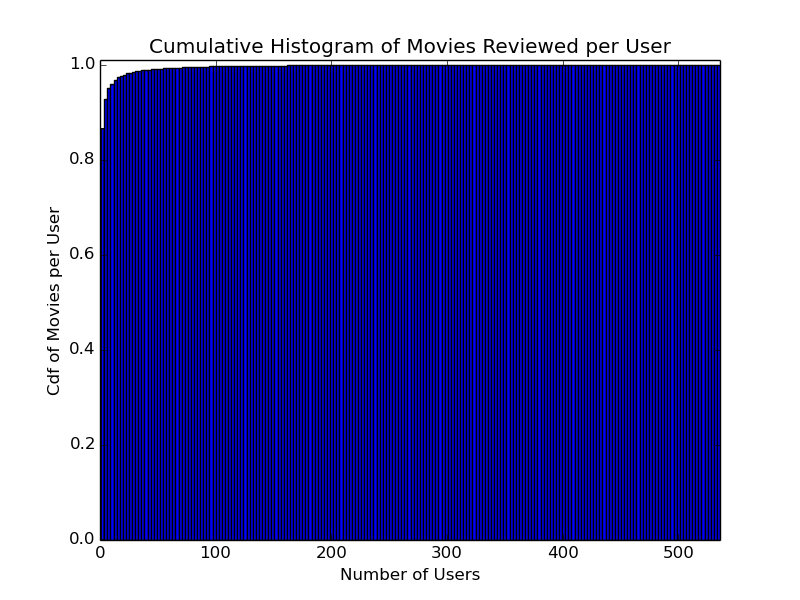
\includegraphics[width=0.48\textwidth]{plots/plot_m_crit_usr.png}
	    \caption{INSERT TITLE}
	    \label{fig:m_crit}
	\end{figure}

\section{Matrix factorization}

	\begin{figure}[H]
	\centering
	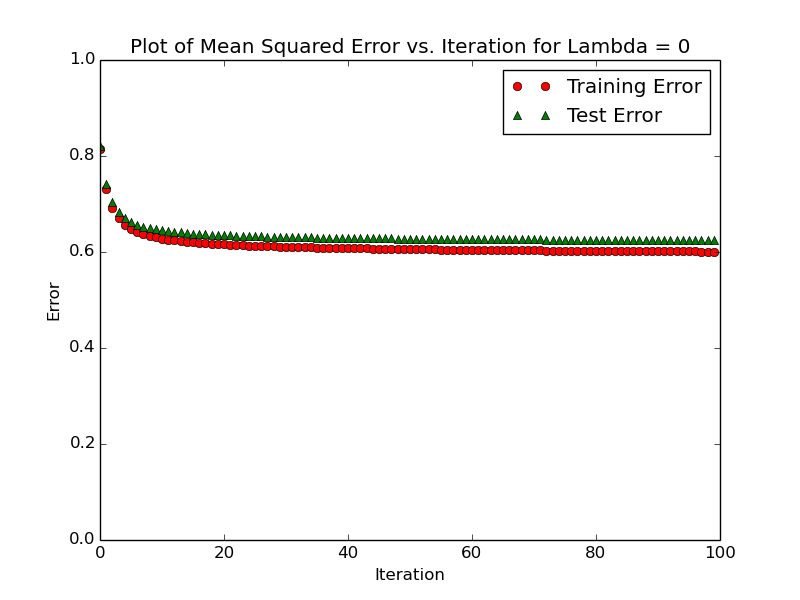
\includegraphics[width=0.48\textwidth]{plots/test-i100d1l0.png}
	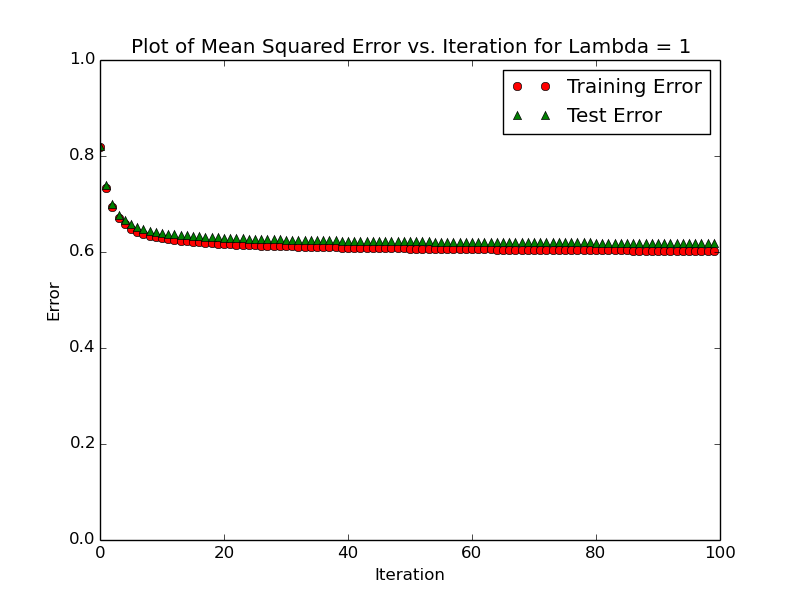
\includegraphics[width=0.48\textwidth]{plots/test-i100d1l1.png}
	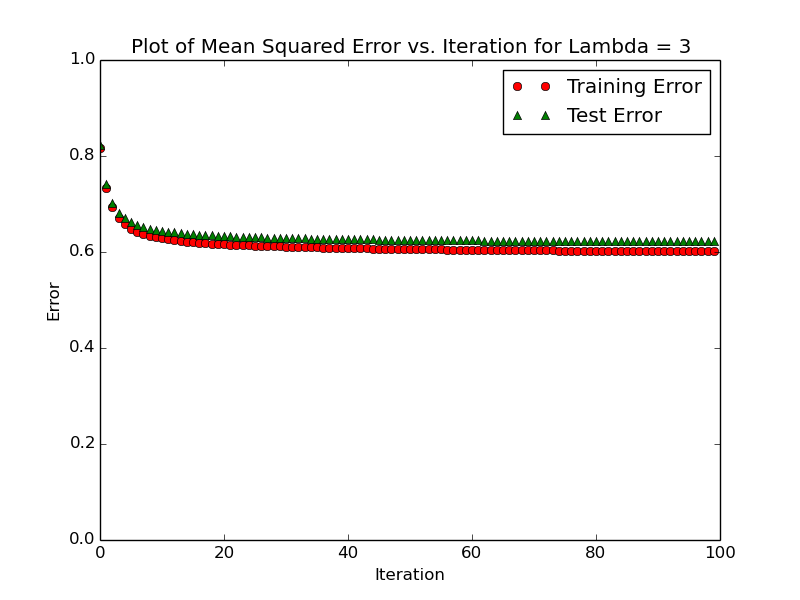
\includegraphics[width=0.48\textwidth]{plots/test-i100d1l3.png}
	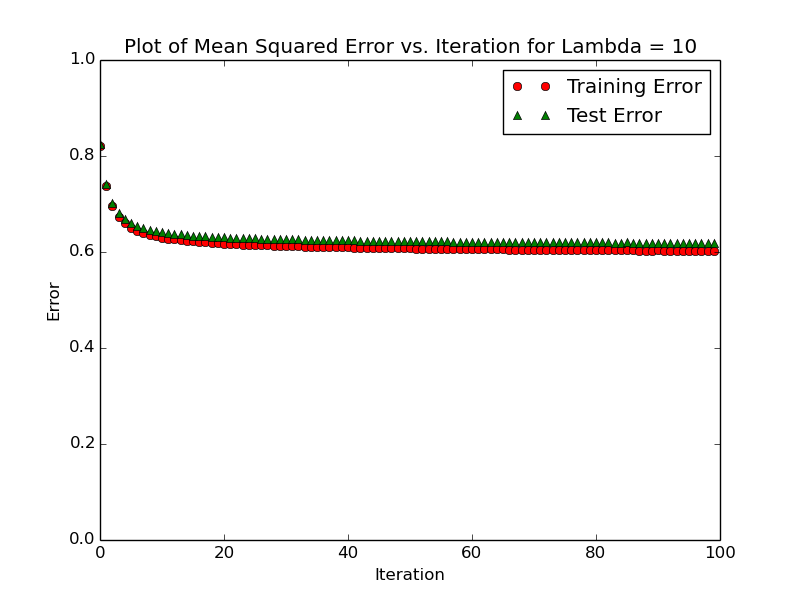
\includegraphics[width=0.48\textwidth]{plots/test-i100d1l10.png}
	\caption{Mean squared training and test error over 100 iterations in the stochastic matrix factorization model. Stocastic gradient descent was done using a step size of 0.02. The learned critic matrix was count(critics) by 1, and the learned movie matrix was 1 by count(movies).}
	\label{fig:1}
	\end{figure}


	\begin{figure}[H]
	\centering
	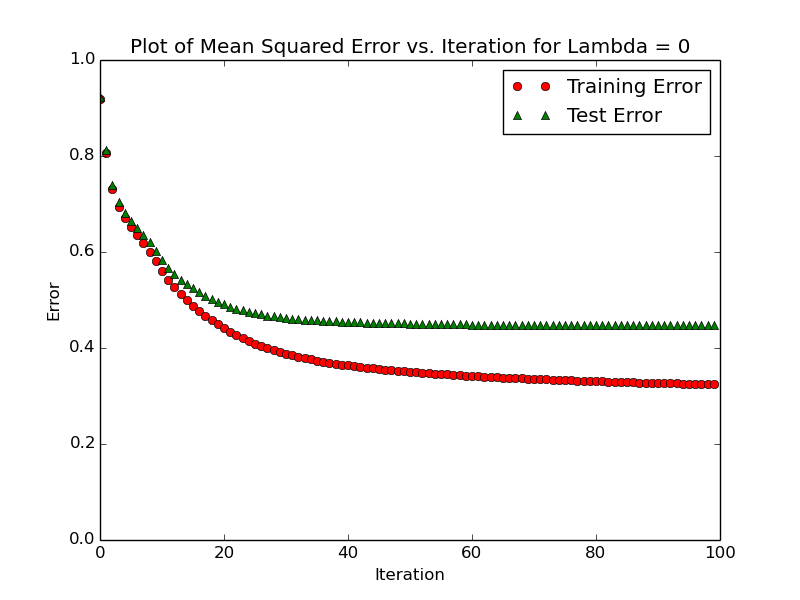
\includegraphics[width=0.48\textwidth]{plots/test-i100d10l0.png}
	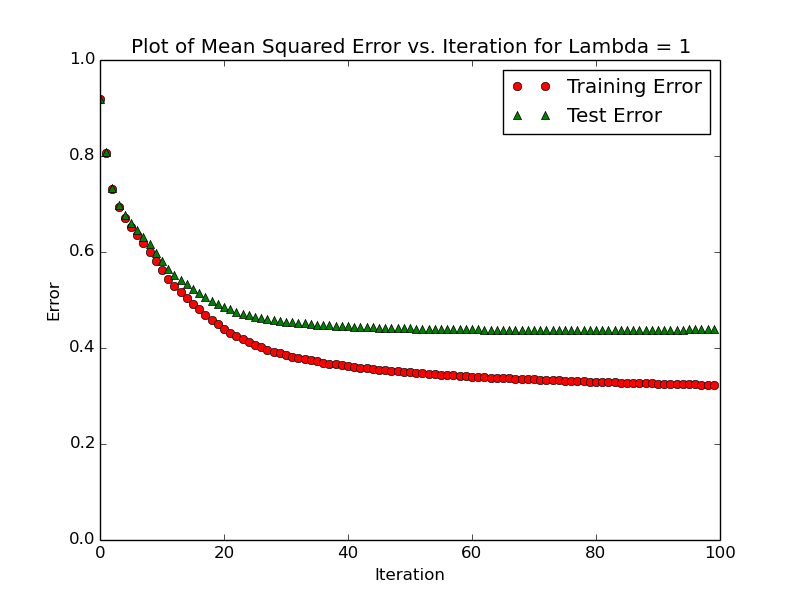
\includegraphics[width=0.48\textwidth]{plots/test-i100d10l1.png}
	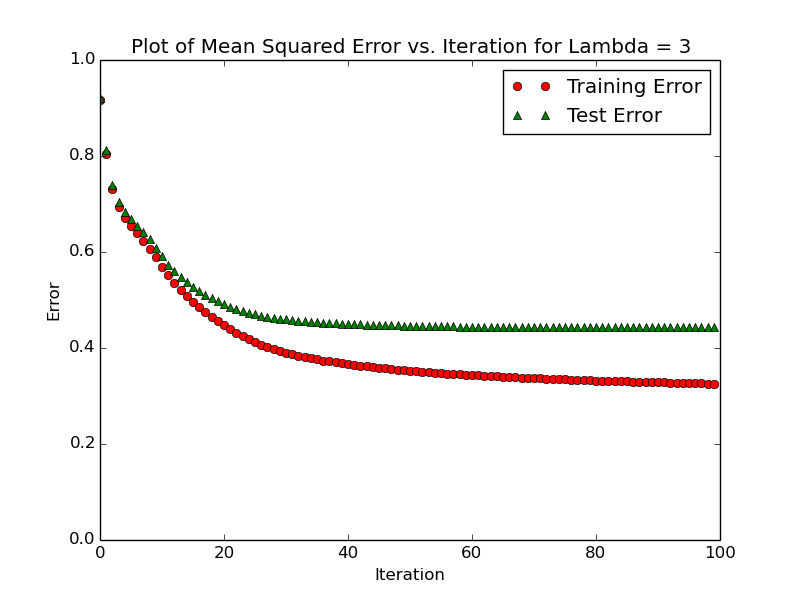
\includegraphics[width=0.48\textwidth]{plots/test-i100d10l3.png}
	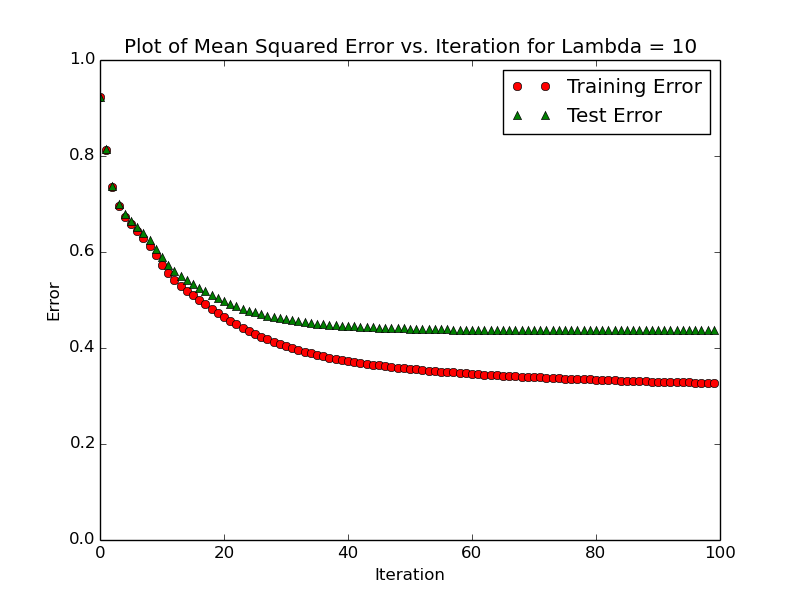
\includegraphics[width=0.48\textwidth]{plots/test-i100d10l10.png}
	\caption{Mean squared training and test error over 100 iterations in the stochastic matrix factorization model. Stocastic gradient descent was done using a step size of 0.02. The learned critic matrix was count(critics) by 10, and the learned movie matrix was 10 by count(movies).}
	\label{fig:10}
	\end{figure}


	\begin{figure}[H]
	\centering
	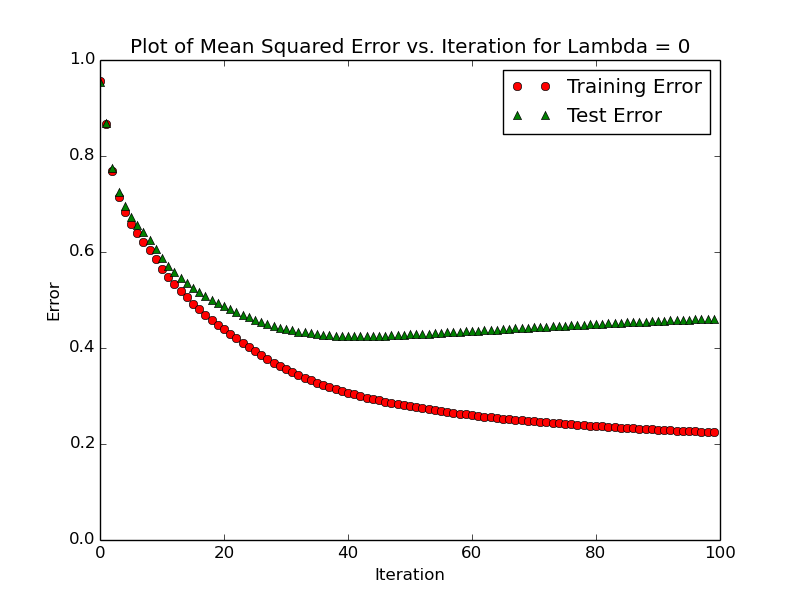
\includegraphics[width=0.48\textwidth]{plots/test-i100d25l0.png}
	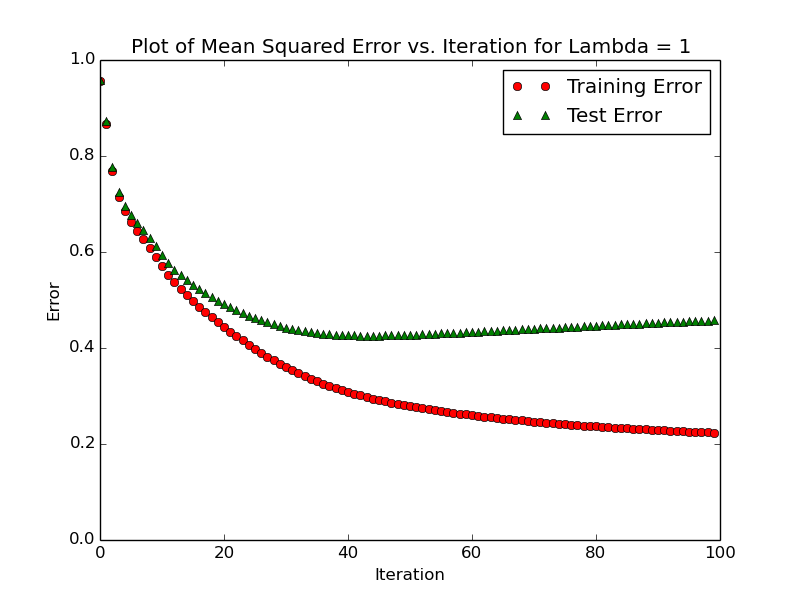
\includegraphics[width=0.48\textwidth]{plots/test-i100d25l1.png}
	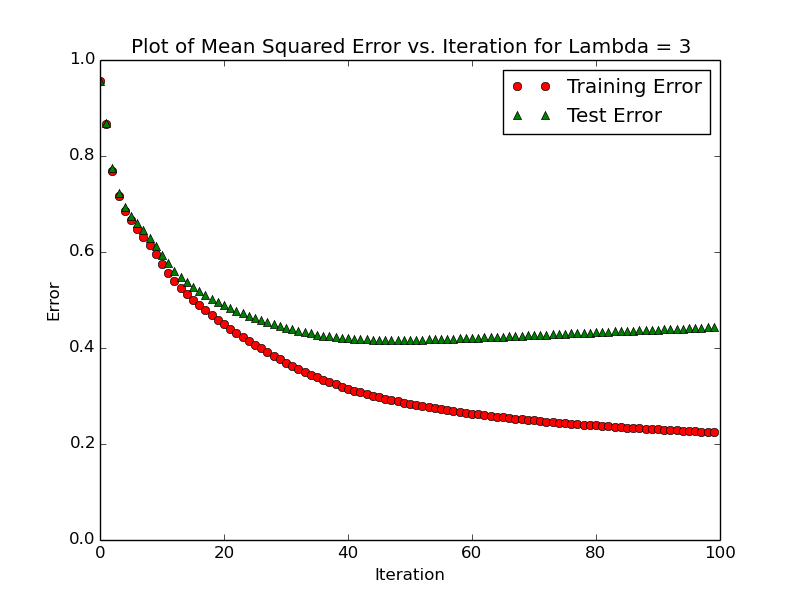
\includegraphics[width=0.48\textwidth]{plots/test-i100d25l3.png}
	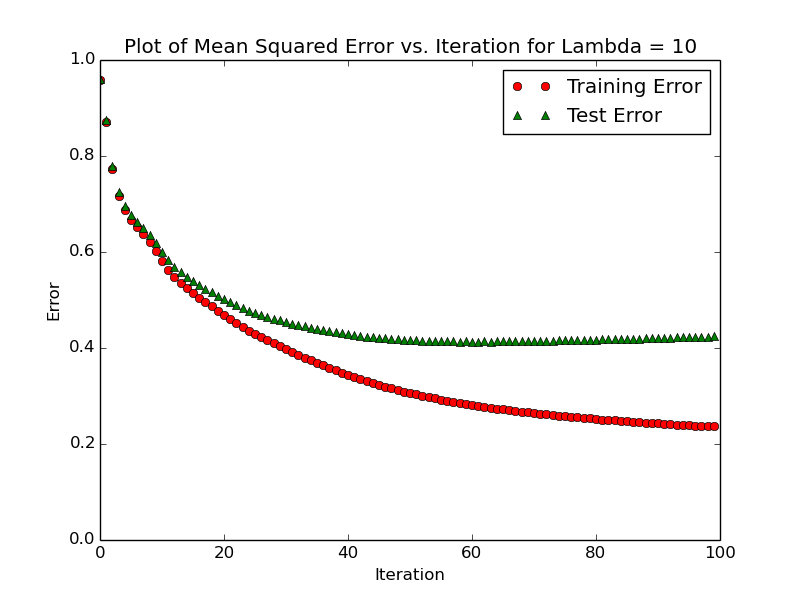
\includegraphics[width=0.48\textwidth]{plots/test-i100d25l10.png}
	\caption{Mean squared training and test error over 100 iterations in the stochastic matrix factorization model. Stocastic gradient descent was done using a step size of 0.02. The learned critic matrix was count(critics) by 25, and the learned movie matrix was 25 by count(movies).}
	\label{fig:25}
	\end{figure}


	\begin{figure}[H]
	\centering
	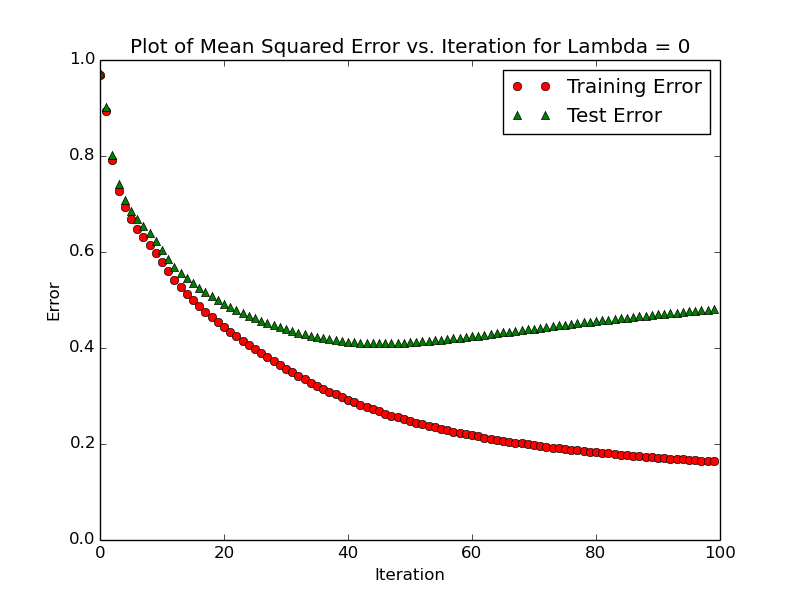
\includegraphics[width=0.48\textwidth]{plots/test-i100d40l0.png}
	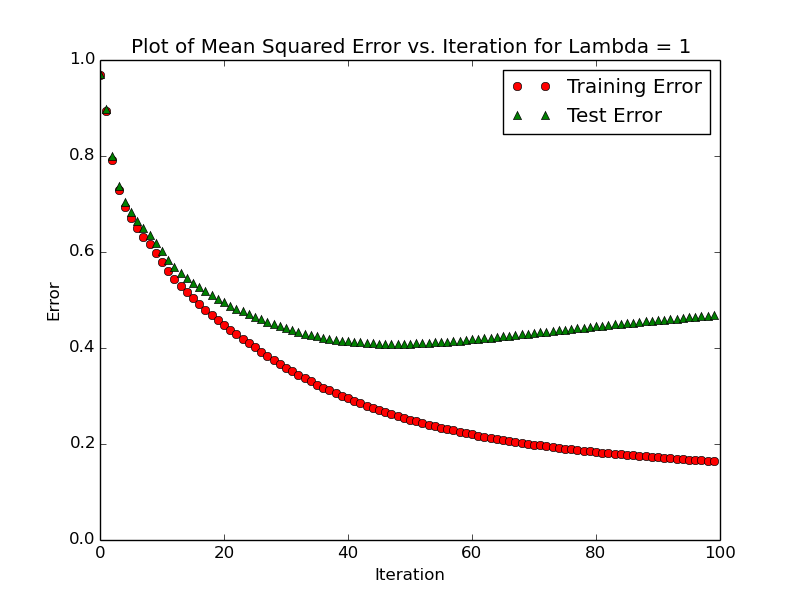
\includegraphics[width=0.48\textwidth]{plots/test-i100d40l1.png}
	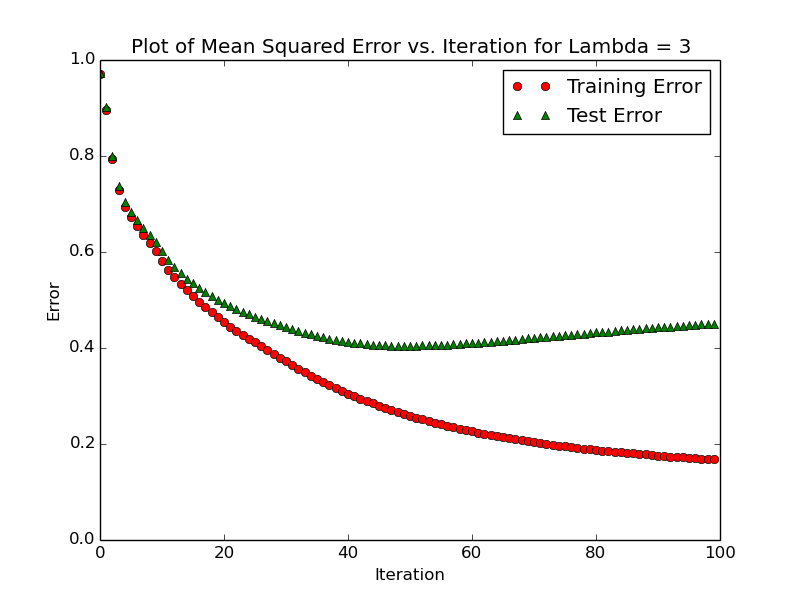
\includegraphics[width=0.48\textwidth]{plots/test-i100d40l3.png}
	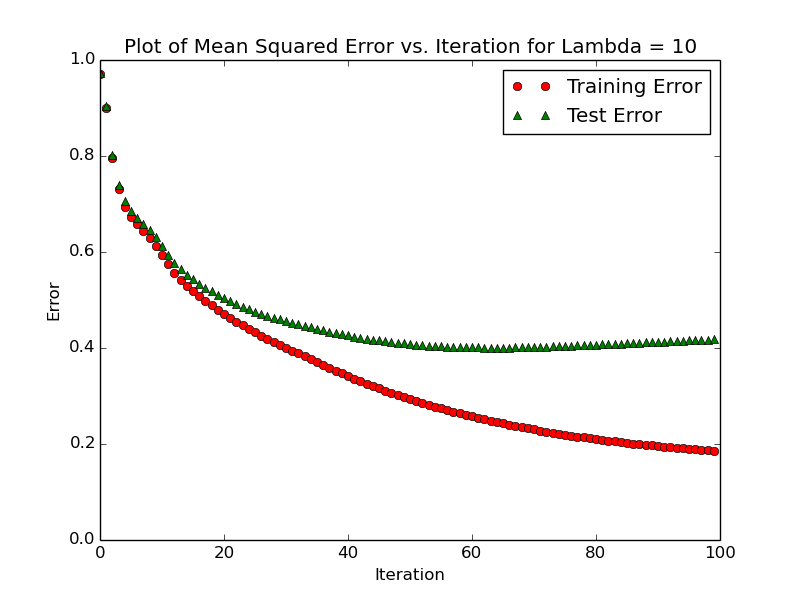
\includegraphics[width=0.48\textwidth]{plots/test-i100d40l10.png}
	\caption{Mean squared training and test error over 100 iterations in the stochastic matrix factorization model. Stocastic gradient descent was done using a step size of 0.02. The learned critic matrix was count(critics) by 40, and the learned movie matrix was 40 by count(movies).}
	\label{fig:40}
	\end{figure}


\section{Recommender Systems}
    
\section{Further work}

\end{document}